\chapter{Diagram class}

\section{User Interface}
		\subsection{Web}
		
	
\section{HTTP}
%begin core diagram
\newpage
\section{Core}
	\subsection{Exercise}
		\begin{figure}[ht]
			\begin{center}
				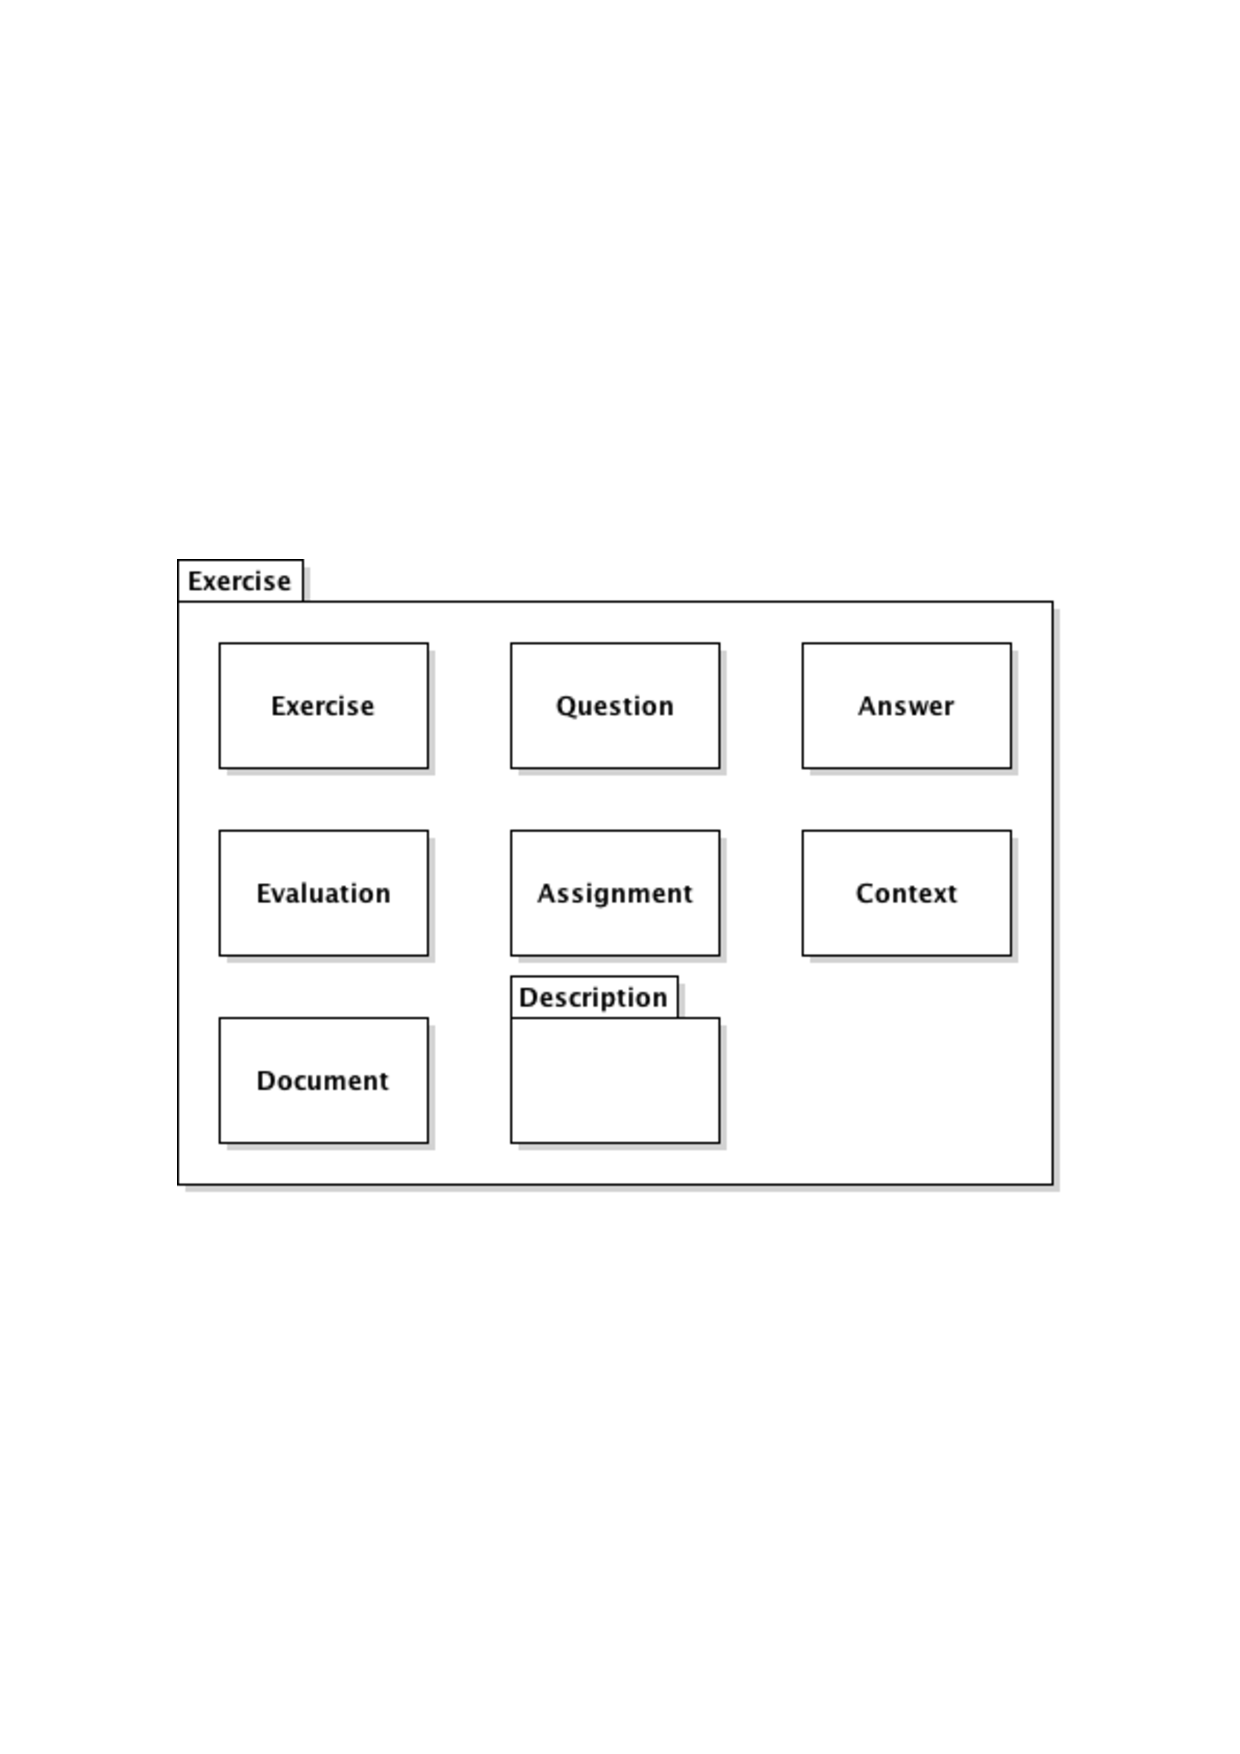
\includegraphics[width=\textwidth,  trim=2cm 9cm 2cm 9cm]{UML_figure/DC/core/exercise/DC_Exercise.pdf}
				\caption{Exercise diagram class : Overview}
			\end{center}
		\end{figure}
	\subsection{Machinist}
		\begin{figure}[ht]
			\begin{center}
				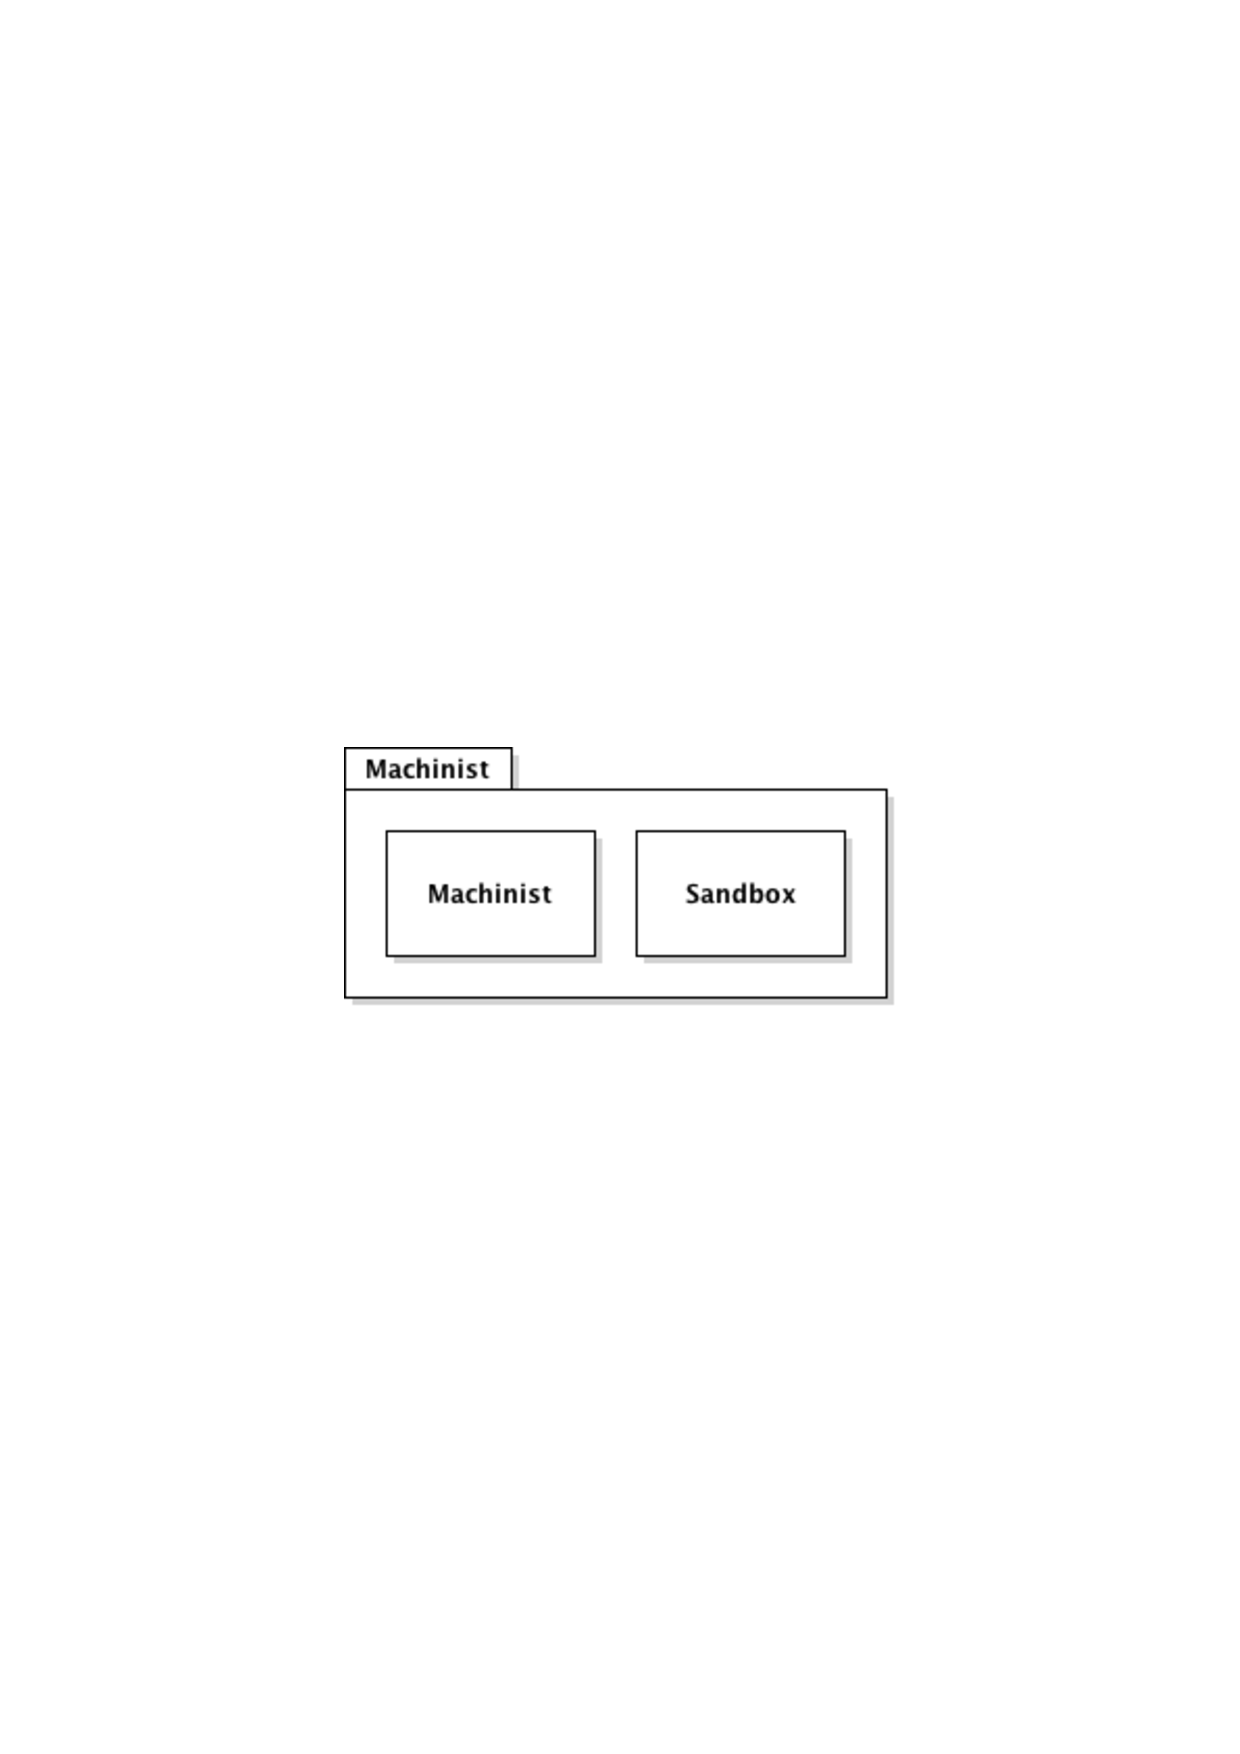
\includegraphics[width=\textwidth,  trim=2cm 12cm 2cm 12cm]{UML_figure/DC/core/machinist/DC_Machinist.pdf}
				\caption{Machinist diagram class : Overview}
			\end{center}
		\end{figure}
\newpage
	\subsection{Reactive}
		\begin{figure}[ht]
			\begin{center}
				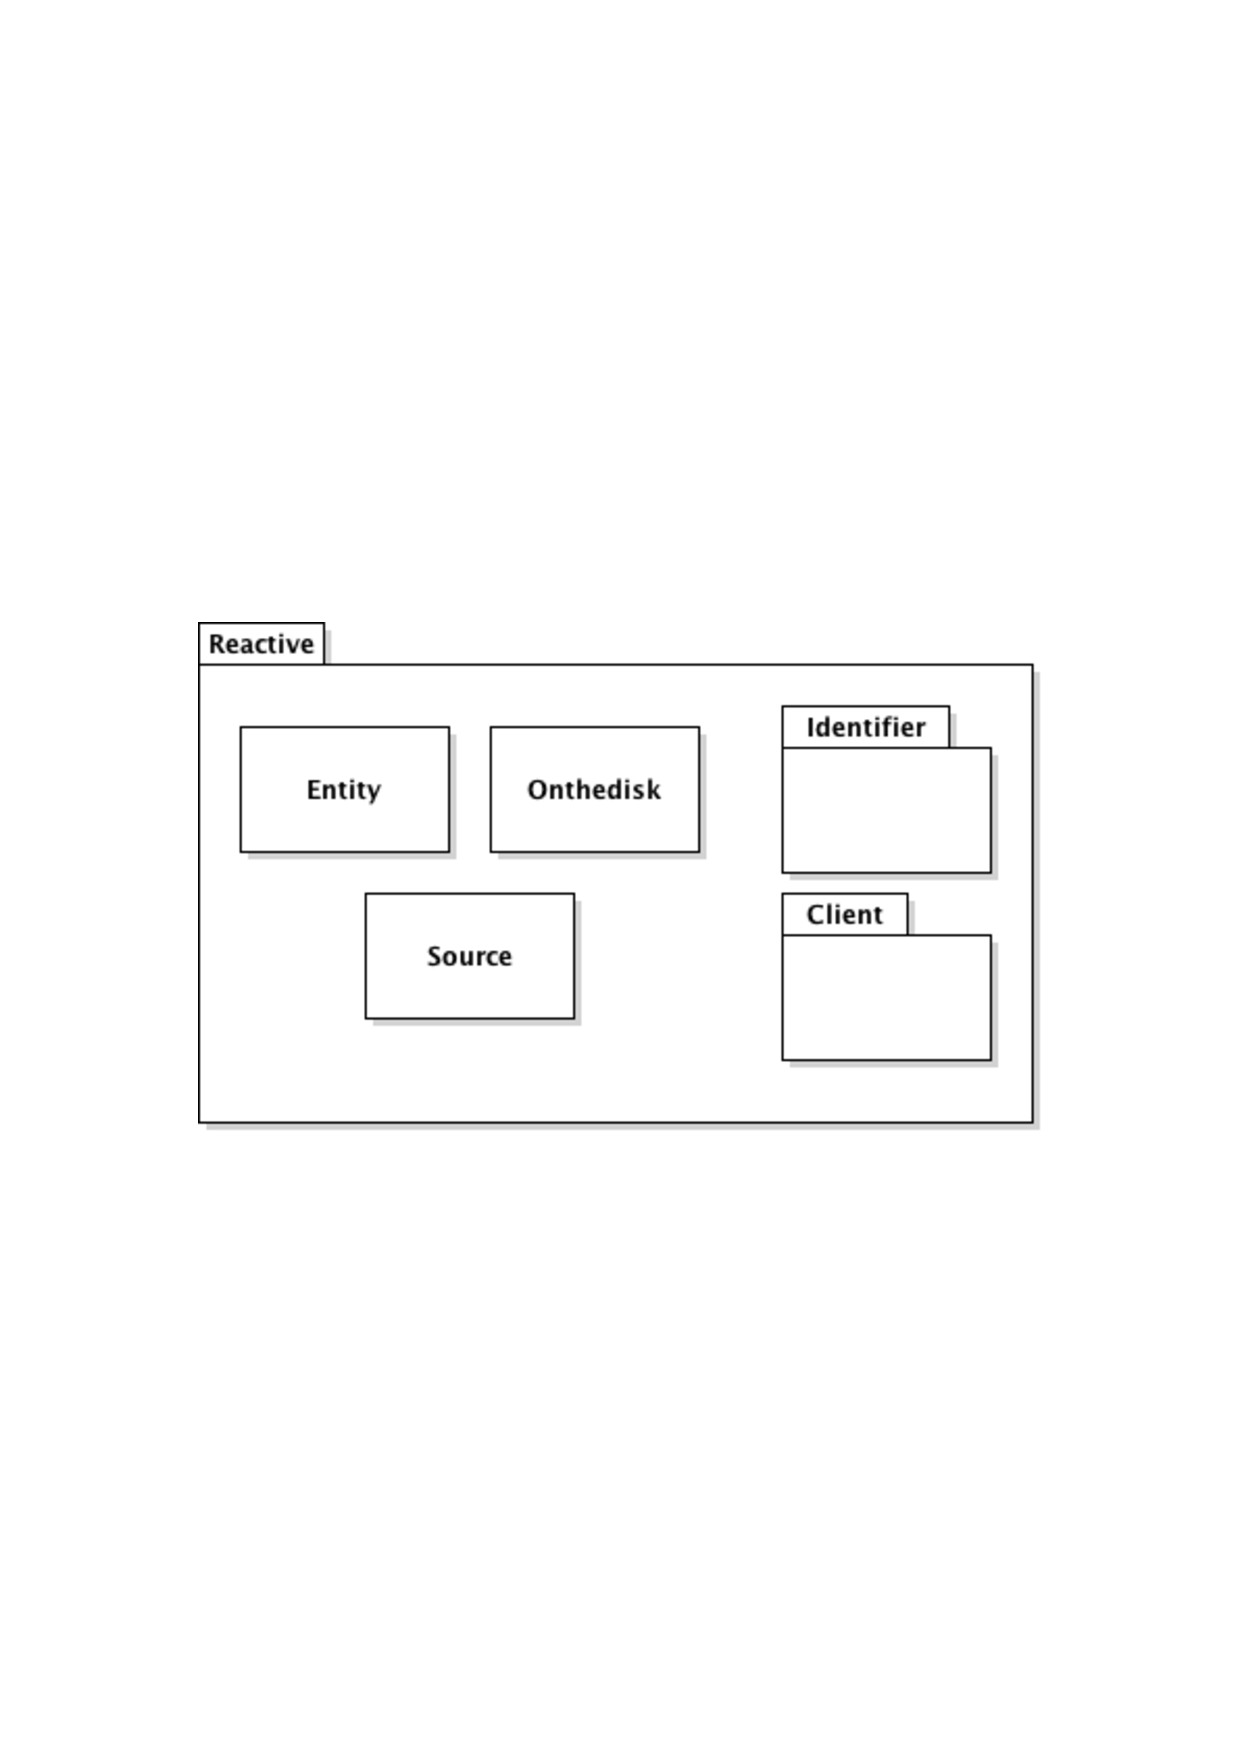
\includegraphics[width=\textwidth,  trim=2cm 10cm 2cm 10cm]{UML_figure/DC/core/reactive/DC_Reactive.pdf}
				\caption{Reactive diagram class : Overview}
			\end{center}
		\end{figure}
	\subsection{Reactive : Identifier}
		\begin{figure}[ht]
			\begin{center}
				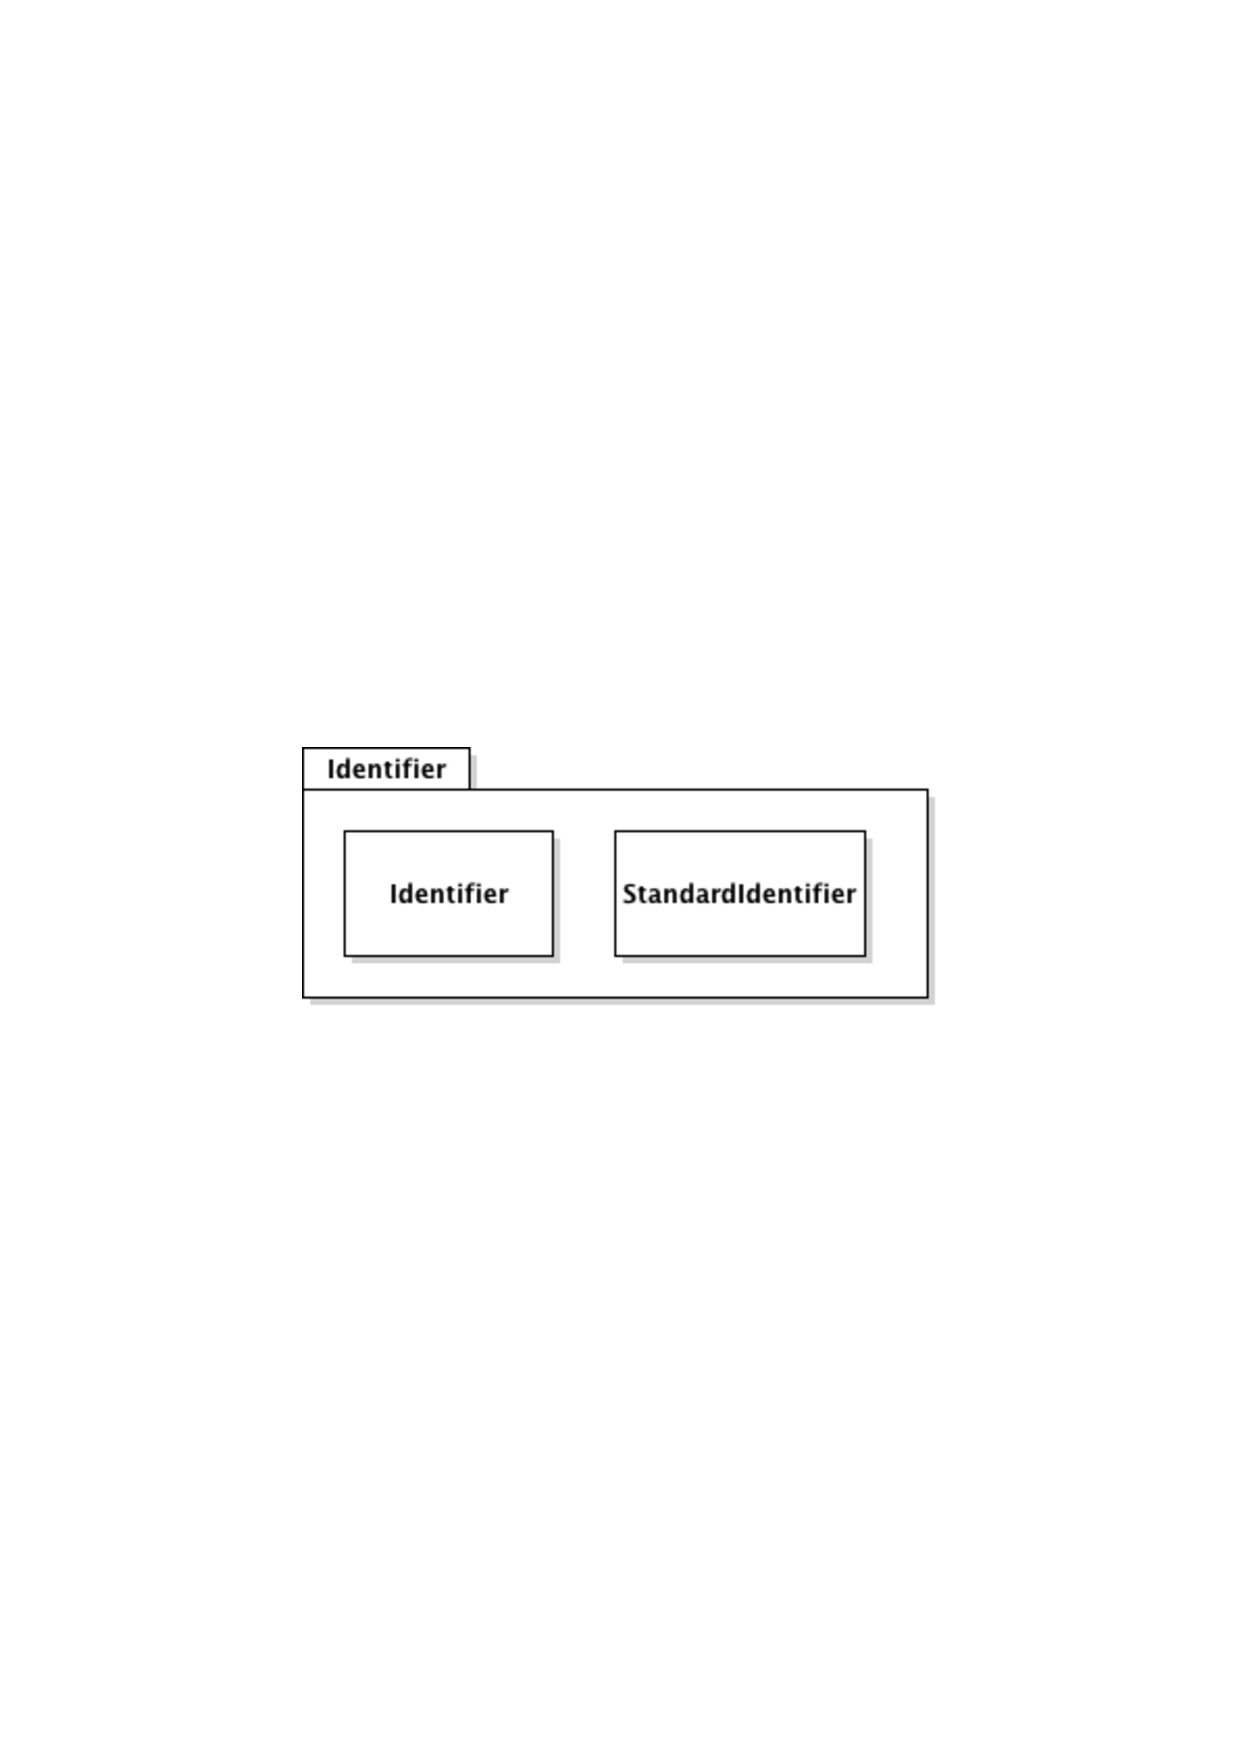
\includegraphics[width=\textwidth,  trim=2cm 12cm 2cm 12cm]{UML_figure/DC/core/reactive/DC_Identifier.pdf}
				\caption{Reactive diagram class : Identifier}
			\end{center}
		\end{figure}
\newpage
	\subsection{Reactive : Client}
		\begin{figure}[ht]
			\begin{center}
				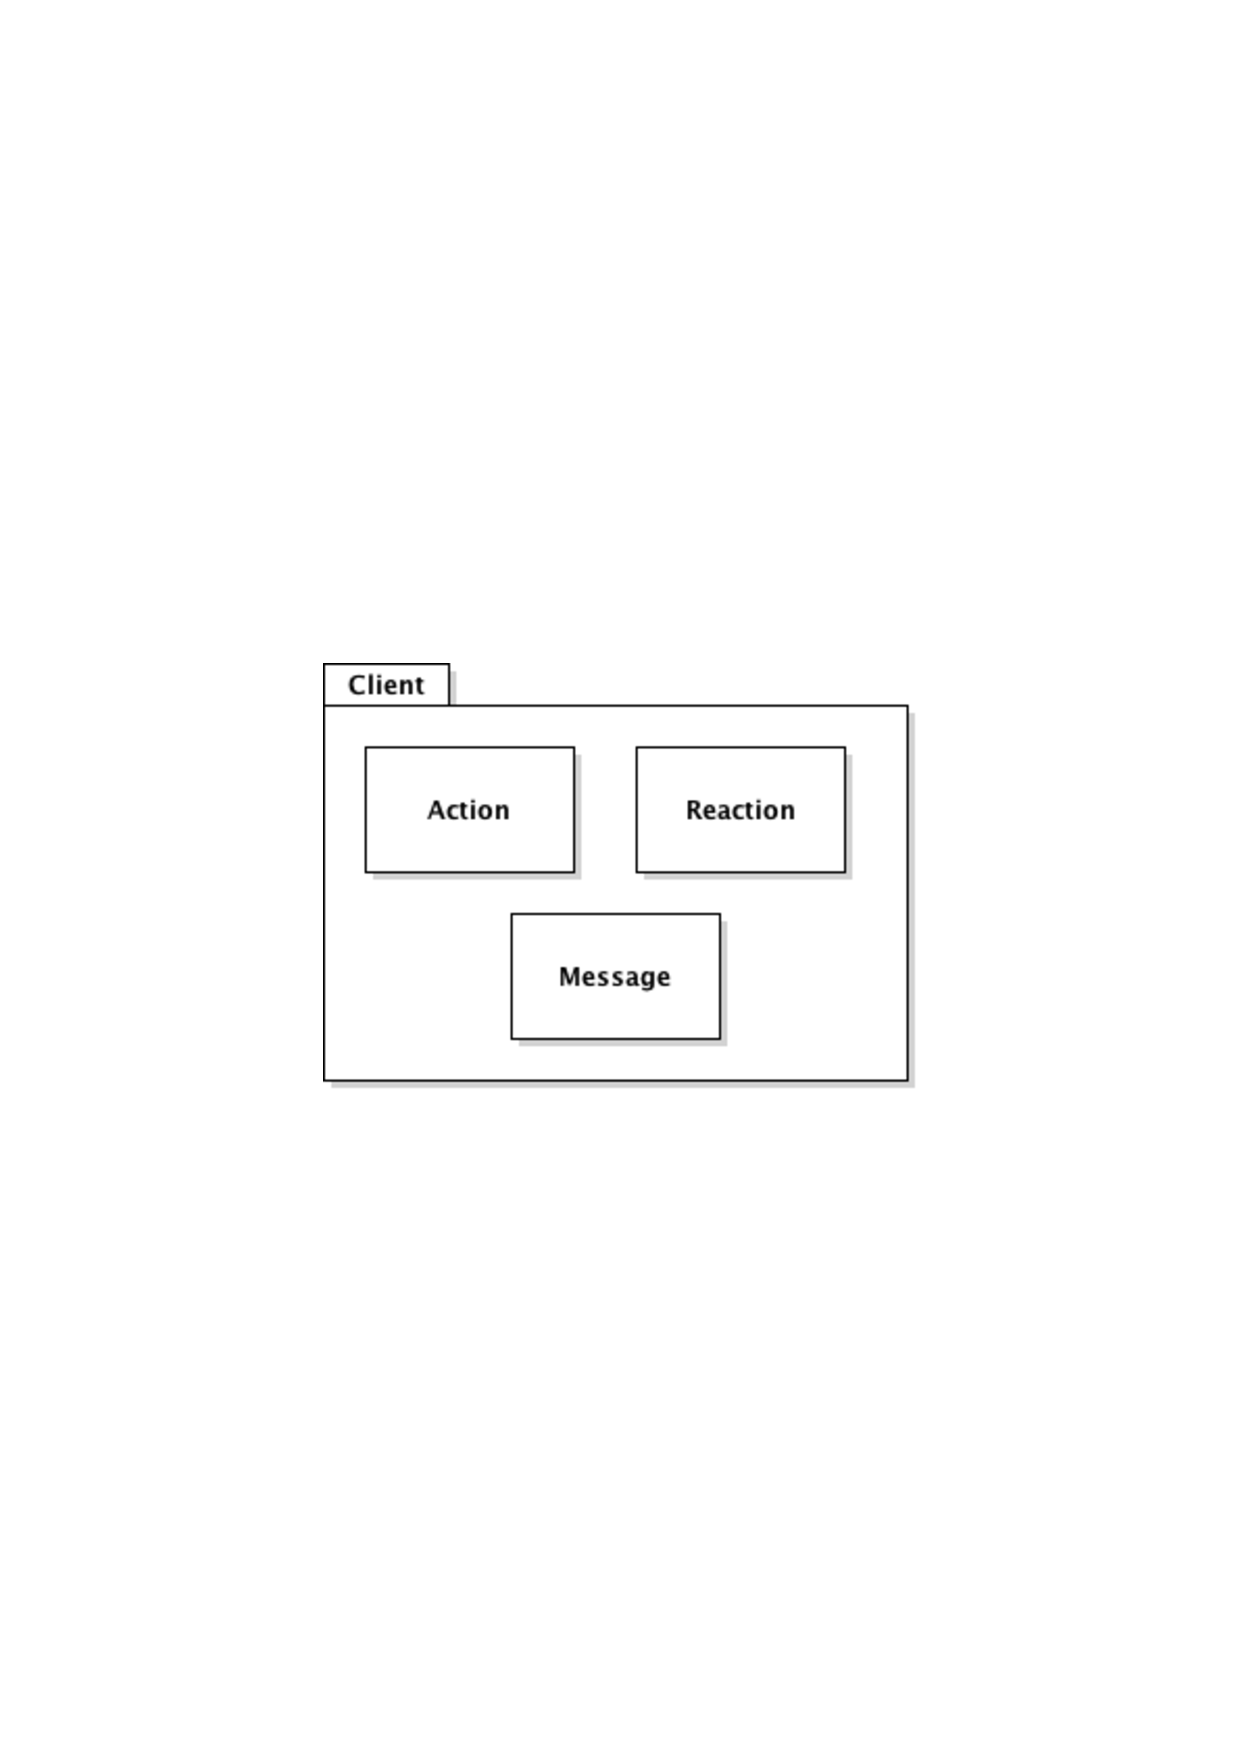
\includegraphics[width=\textwidth,  trim=2cm 11cm 2cm 10cm]{UML_figure/DC/core/reactive/DC_Client.pdf}
				\caption{Reactive diagram class : Client}
			\end{center}
		\end{figure}
	\subsection{User}
		\begin{figure}[ht]
			\begin{center}
				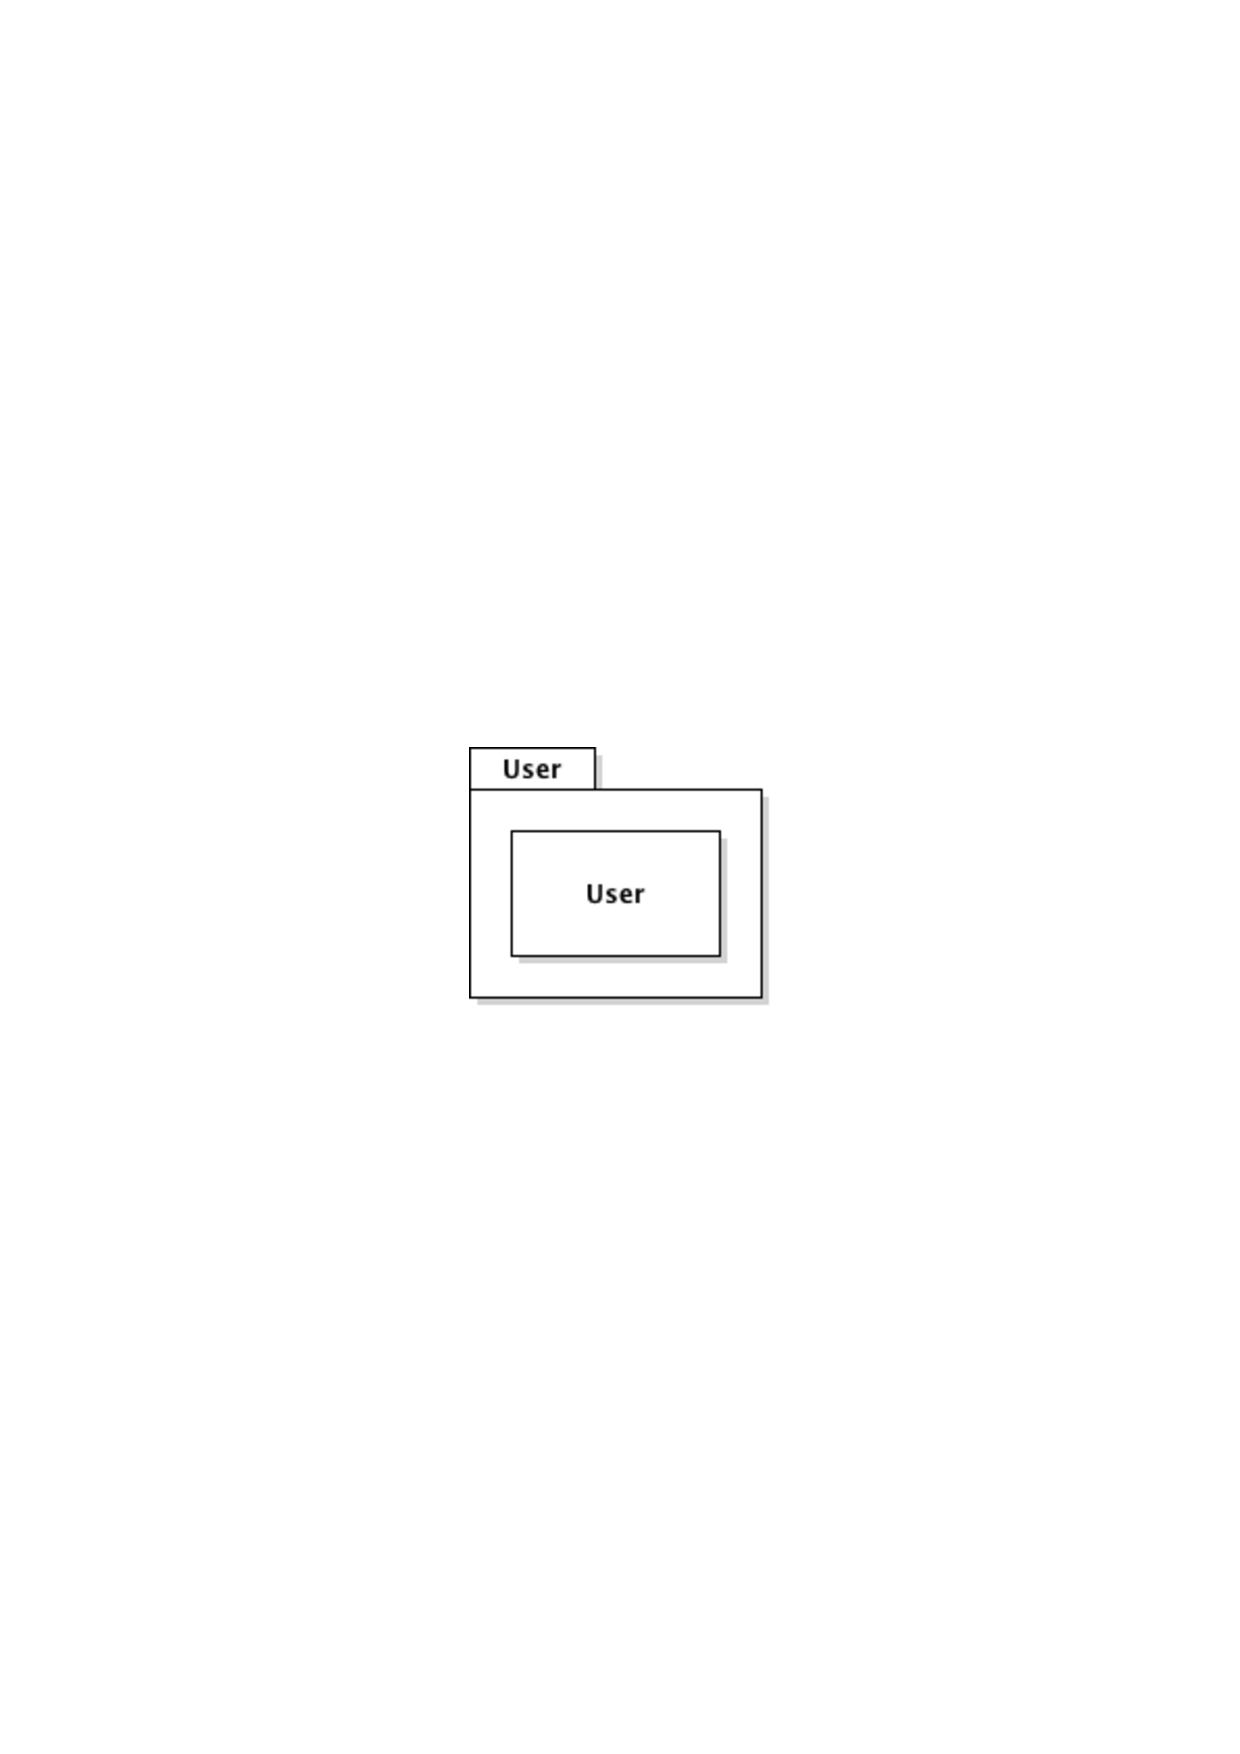
\includegraphics[width=\textwidth,  trim=2cm 12cm 2cm 12cm]{UML_figure/DC/core/user/DC_User.pdf}
				\caption{User diagram class : Overview}
			\end{center}
		\end{figure}
\newpage
	\subsection{Config}
		\begin{figure}[ht]
			\begin{center}
				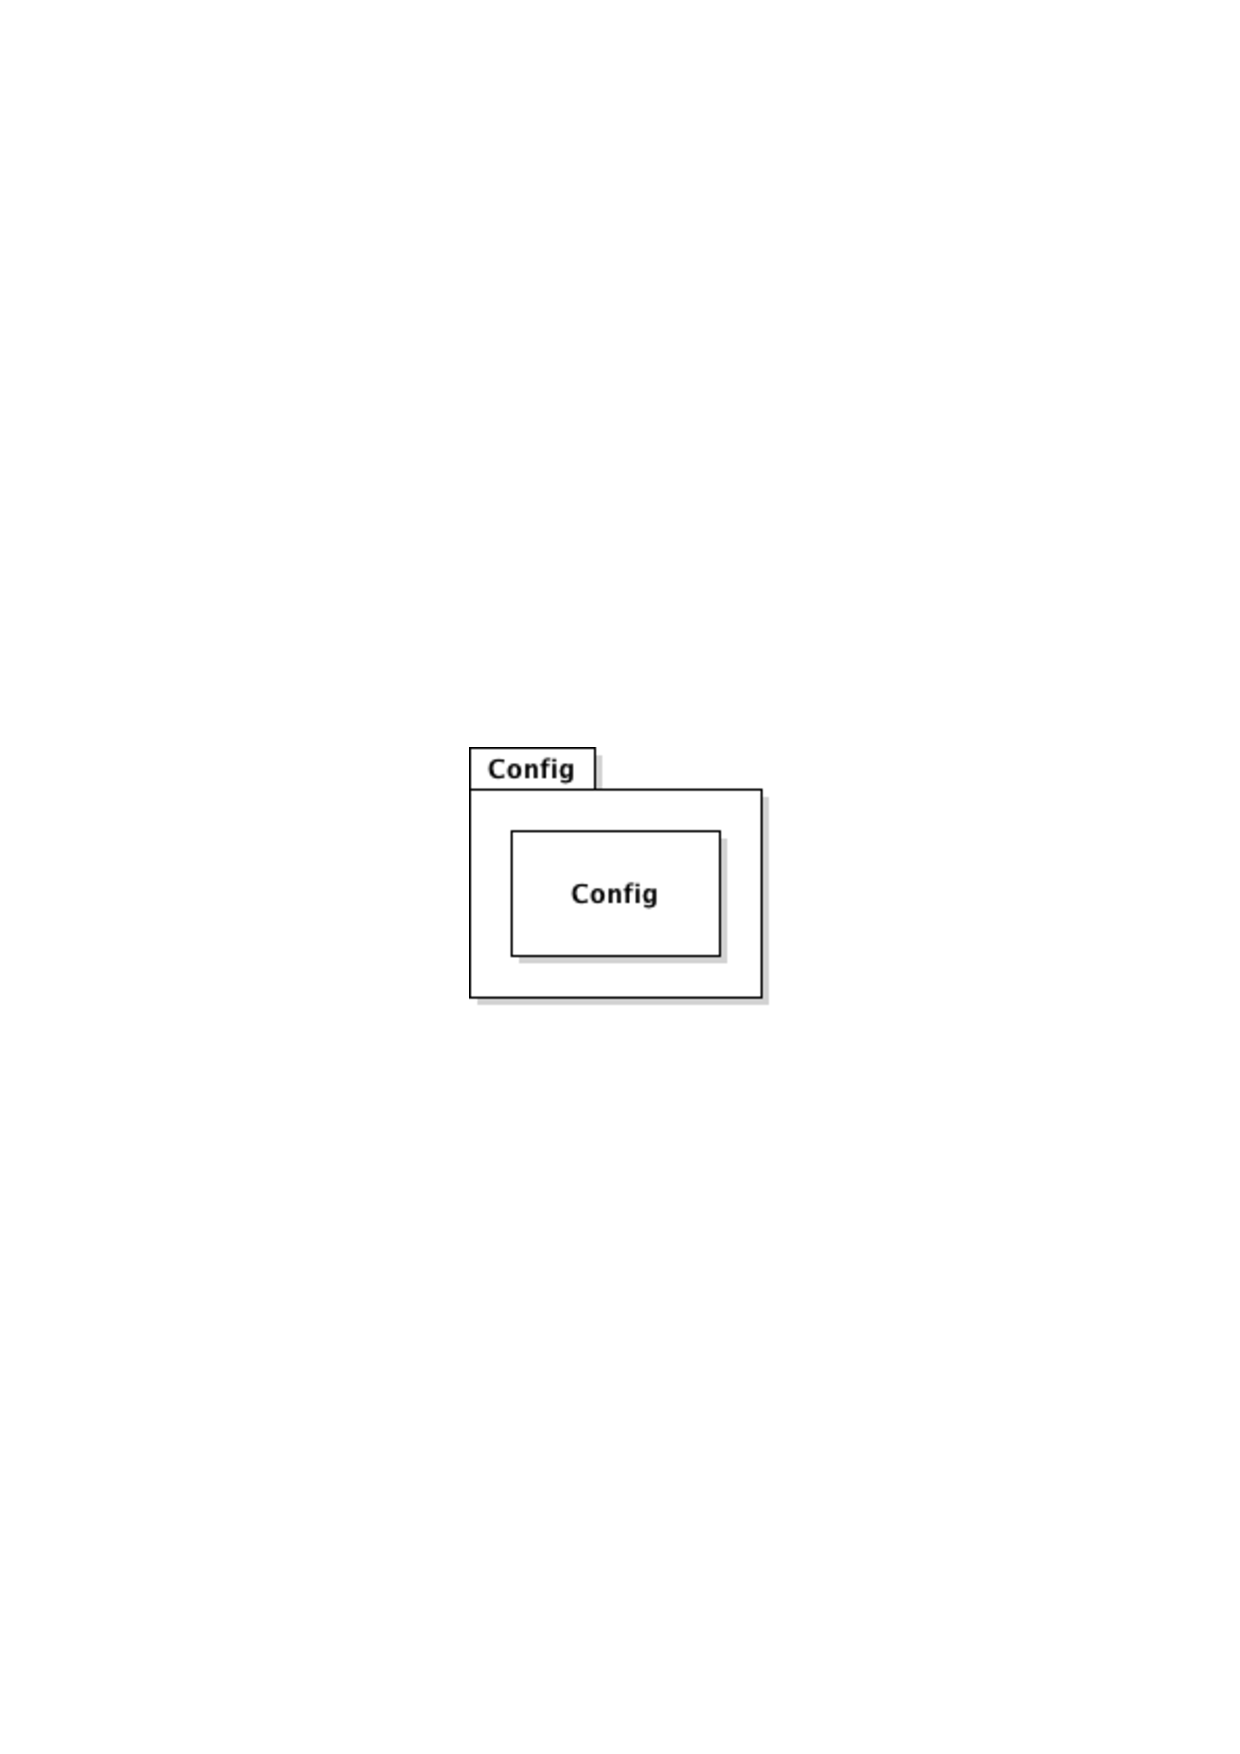
\includegraphics[width=\textwidth,  trim=2cm 12cm 2cm 12cm]{UML_figure/DC/core/config/DC_Config.pdf}
				\caption{Config diagram class : Overview}
			\end{center}
		\end{figure}
	\subsection{Errors}
	\subsection{Common}

%end core diagram
\newpage
\section{Common}
	\begin{figure}[ht]
			\begin{center}
				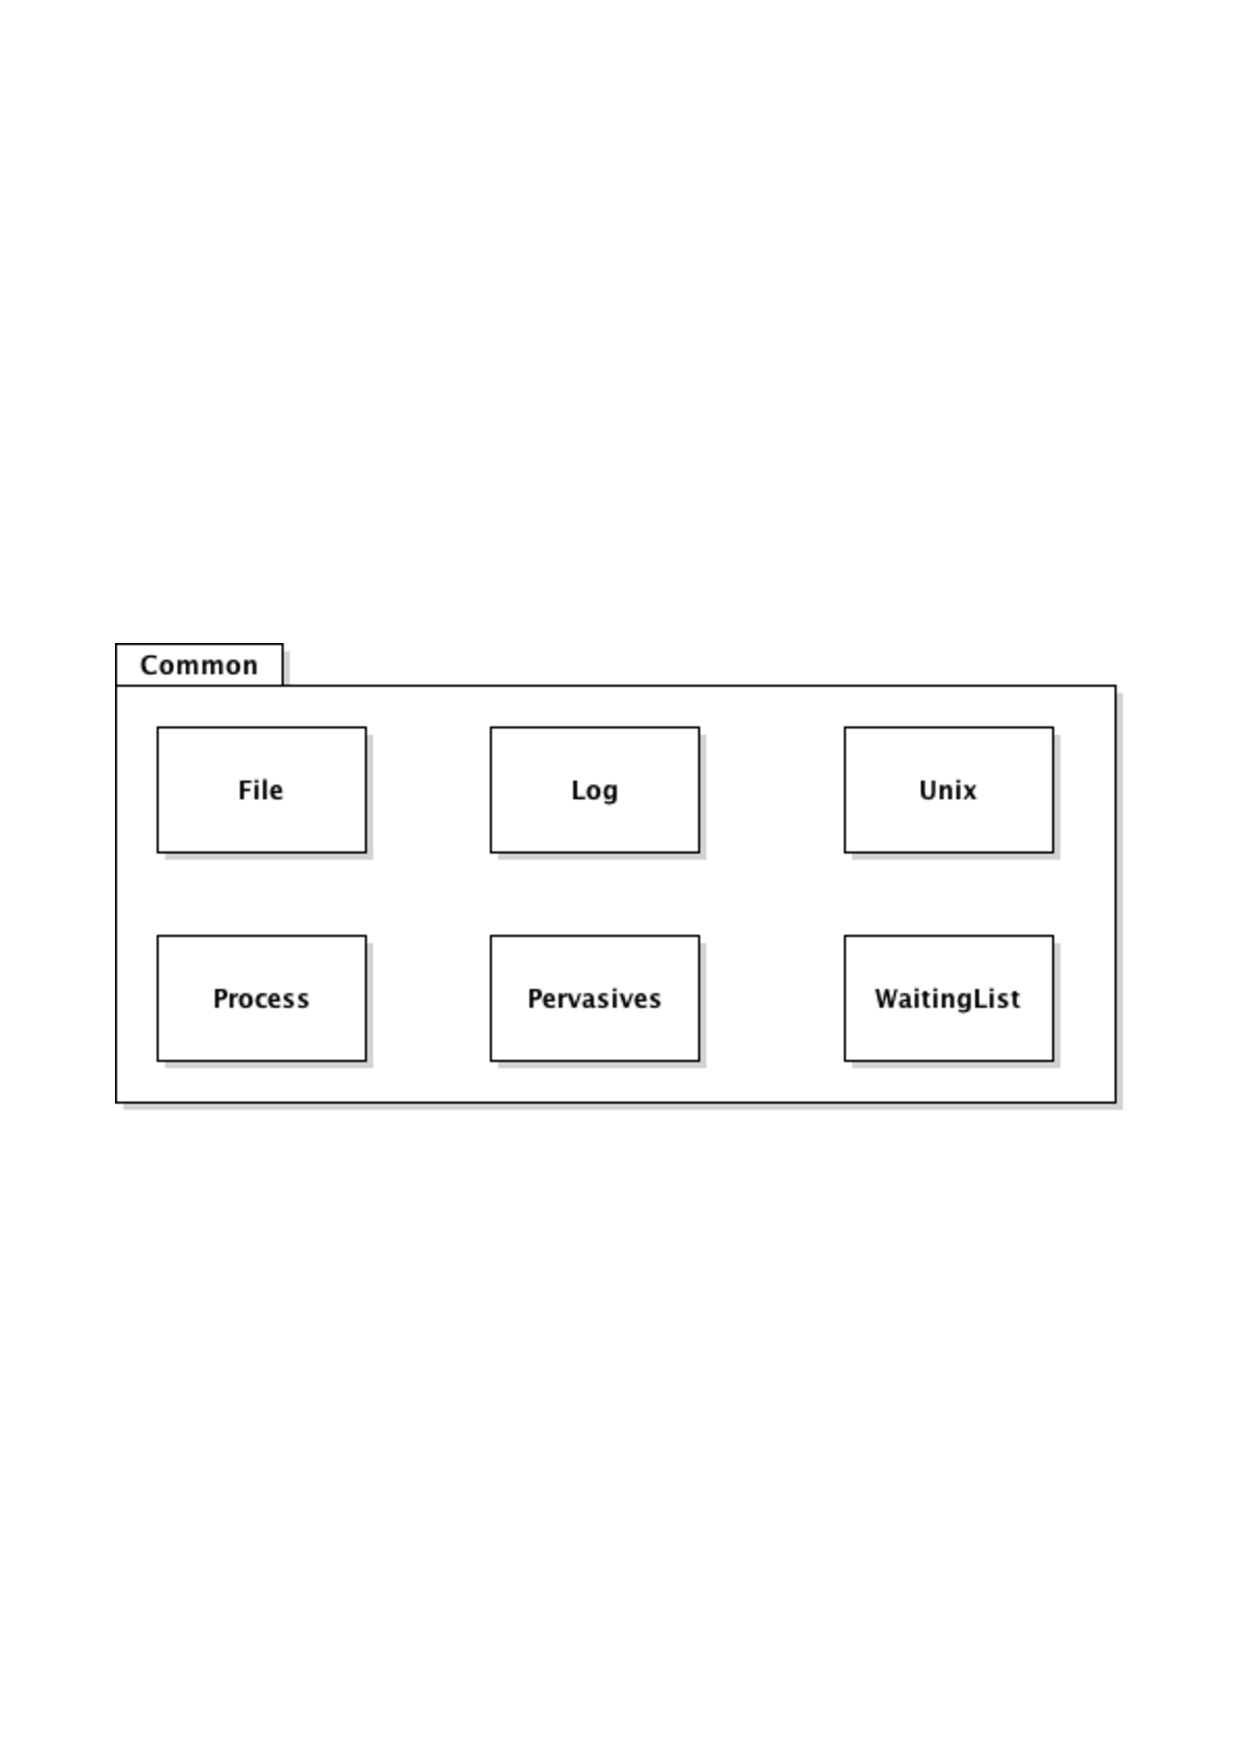
\includegraphics[width=\textwidth,  trim=2cm 10cm 2cm 11cm]{UML_figure/DC/common/DC_Common.pdf}
				\caption{Common diagram class : Overview}
			\end{center}
		\end{figure}







